% =====================================================================
%  Desenhos técnicos do DAD01 em vetor (TikZ) — estilo de desenho técnico
%  Medidas em mm.
% =====================================================================

\definecolor{fiomarrom}{HTML}{7B4A26}
\definecolor{fiolaranja}{HTML}{F08A1C}
\definecolor{fioverde}{HTML}{2E9E3E}
\definecolor{fiovermelho}{HTML}{D42A2A}
\definecolor{tdline}{HTML}{262626}
\definecolor{tdfill}{HTML}{F2F2F2}
\definecolor{tddim}{HTML}{4D4D4D}

\tikzset{
  td/.style={draw=tdline,line width=0.55pt},
  tdfino/.style={draw=tdline,line width=0.3pt},
  tdoculto/.style={draw=tdline!70,line width=0.3pt,dash pattern=on 1.2pt off 0.8pt},
  tdeixo/.style={draw=tdline!60,line width=0.25pt,dash pattern=on 4pt off 1pt on 0.6pt off 1pt},
  cota/.style={tddim,line width=0.3pt,{Stealth[length=1.5mm,width=0.8mm]}-{Stealth[length=1.5mm,width=0.8mm]}},
  aux/.style={tddim,line width=0.25pt},
  rot/.style={font=\scriptsize,text=tdline,fill=white,inner sep=0.8pt},
  vista/.style={font=\tiny\bfseries,text=tddim},
  chamada/.style={circle,draw=tdline,line width=0.4pt,fill=white,font=\tiny\bfseries,inner sep=0pt,minimum size=3.6mm},
  lider/.style={tdline,line width=0.3pt},
}

% ---------------- Unidade exposta: vistas frontal e lateral ----------------
\newcommand{\desenhoExposta}{%
\begin{tikzpicture}[x=0.36mm,y=0.36mm]
  % vista frontal
  \draw[td,fill=white,rounded corners=0.6mm] (-8.5,84.4) rectangle (0,94.9);           % bocal
  \draw[td,fill=white,rounded corners=2mm] (0,0) rectangle (62.3,112.5);
  \draw[tdfino,rounded corners=0.8mm] (6.7,31.1) rectangle (55.6,104.5);              % moldura da tela
  \draw[tdfino,fill=tdfill] (9,34) rectangle (53.3,101.6);                            % área ativa
  \node[font=\tiny\itshape\bfseries,text=tdline!60] at (31.15,15) {SIGHIR};
  % vista lateral
  \draw[td,fill=white,rounded corners=1.6mm] (80,0) rectangle (109,112.5);
  \draw[tdfino] (84,4) -- (84,108.5);
  \draw[tdoculto] (80,84.4) -- (109,84.4); \draw[tdoculto] (80,94.9) -- (109,94.9);
  % cotas
  \draw[aux] (0,114) -- (0,123); \draw[aux] (62.3,114) -- (62.3,123);
  \draw[cota] (0,120) -- node[rot]{62,3} (62.3,120);
  \draw[aux] (80,114) -- (80,123); \draw[aux] (109,114) -- (109,123);
  \draw[cota] (80,120) -- node[rot]{29,0} (109,120);
  \draw[aux] (110.5,0) -- (120,0); \draw[aux] (110.5,112.5) -- (120,112.5);
  \draw[cota] (117,0) -- node[rot,rotate=90]{112,5} (117,112.5);
  \node[vista] at (31.15,-9) {VISTA FRONTAL};
  \node[vista] at (94.5,-9) {VISTA LATERAL};
\end{tikzpicture}}

% ---------------- Unidade embutida: vistas superior e lateral ----------------
\newcommand{\dbnove}[3]{% x, y (base), largura — conector DB9 em vista superior
  \draw[tdfino,fill=white] (#1,#2) rectangle ({#1+#3},{#2+2.2});
  \draw[tdfino,fill=tdfill] ({#1+2.2},{#2+2.2}) -- ({#1+#3-2.2},{#2+2.2}) -- ({#1+#3-3.4},{#2+6.5}) -- ({#1+3.4},{#2+6.5}) -- cycle;}
\newcommand{\desenhoEmbutida}{%
\begin{tikzpicture}[x=0.33mm,y=0.33mm]
  % vista superior
  \draw[td,fill=white,rounded corners=1mm] (122,24) -- (129,27) -- (129,61) -- (122,64);  % orelha
  \draw[tdfino,rounded corners=0.8mm] (123.5,34) rectangle (126.5,54);
  \draw[td,fill=white,rounded corners=3mm] (0,0) rectangle (122,88);
  \draw[tdfino,rounded corners=2mm] (14,10) rectangle (108,72);
  \dbnove{12}{88}{22}
  \draw[tdfino,fill=white] (44,88) rectangle (56,93);                                   % Microfit 8
  \draw[tdfino,fill=white] (76,88) rectangle (85,93);                                   % Microfit 6
  % vista lateral
  \draw[td,fill=white,rounded corners=1.5mm] (0,-46) rectangle (122,-18);
  \draw[tdfino] (0,-26) -- (122,-26);
  % cotas
  \draw[aux] (0,96) -- (0,106); \draw[aux] (129,63) -- (129,106);
  \draw[cota] (0,103) -- node[rot]{129} (129,103);
  \draw[aux] (-1.5,0) -- (-11,0); \draw[aux] (-1.5,88) -- (-11,88);
  \draw[cota] (-8,0) -- node[rot,rotate=90]{88} (-8,88);
  \draw[aux] (-1.5,-46) -- (-11,-46); \draw[aux] (-1.5,-18) -- (-11,-18);
  \draw[cota] (-8,-46) -- node[rot,rotate=90]{28} (-8,-18);
  \node[vista] at (61,40) {VISTA SUPERIOR};
  \node[vista] at (61,-53) {VISTA LATERAL};
\end{tikzpicture}}

% ---------------- Conector Microfit 6 vias (vista frontal, lado do cabo) ----------------
\newcommand{\desenhoConector}{%
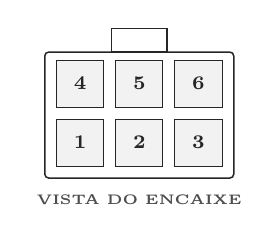
\begin{tikzpicture}[x=1mm,y=1mm]
  \draw[td,fill=white,rounded corners=0.5mm] (-1.5,-1.5) rectangle (22.5,14.5);
  \draw[td,fill=white] (7,14.5) rectangle (14,17.5);                                    % trava
  \foreach \i/\x/\y in {1/0/0, 2/7.5/0, 3/15/0, 4/0/7.5, 5/7.5/7.5, 6/15/7.5} {
    \draw[tdfino,fill=tdfill] (\x,\y) rectangle ({\x+6},{\y+6});
    \node[font=\scriptsize\bfseries,text=tdline] at ({\x+3},{\y+3}) {\i};}
  \node[vista] at (10.5,-4.3) {VISTA DO ENCAIXE};
\end{tikzpicture}}

% ---------------- Diagrama de ligação no veículo ----------------
\newcommand{\figuraIntegracao}{%
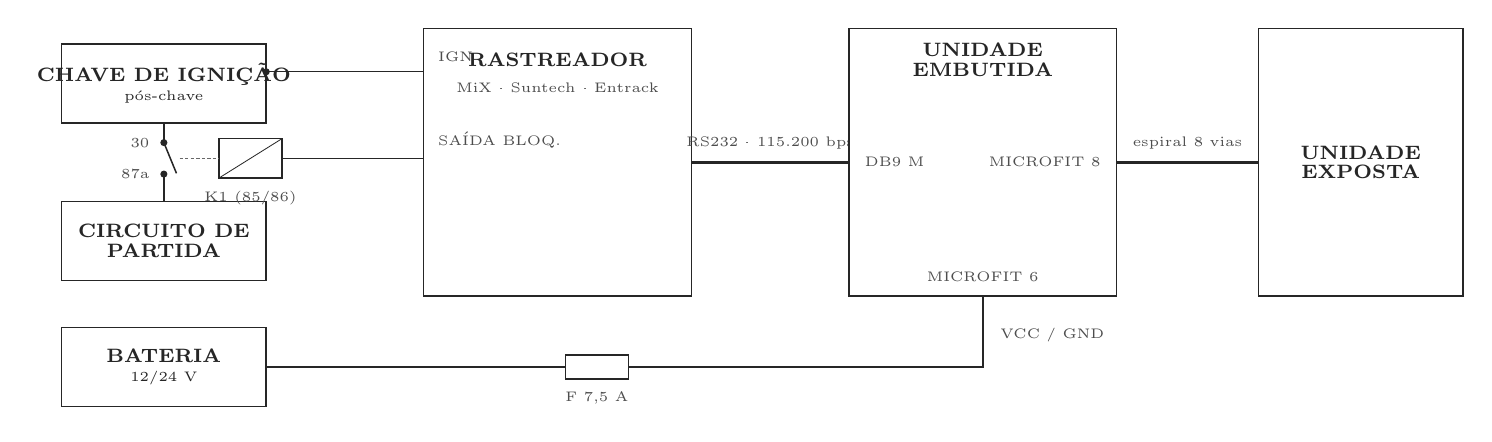
\begin{tikzpicture}[x=1mm,y=1mm,
  bloco/.style={td,fill=white,align=center,font=\scriptsize},
  titb/.style={font=\scriptsize\bfseries,text=tdline,align=center},
  porta/.style={font=\tiny,text=tddim},
  fio/.style={tdline,line width=0.55pt},
  ser/.style={tdline,line width=1.1pt}]
  % --- chave de ignição e relé de bloqueio
  \draw[td,fill=white] (0,30) rectangle (26,40);
  \node[titb] at (13,35) {CHAVE DE IGNIÇÃO\\[-1pt]{\normalfont\tiny pós-chave}};
  \draw[fio] (13,30) -- (13,27.5);
  \fill[tdline] (13,27.5) circle (0.45); \node[porta,anchor=east] at (12.4,27.5) {30};
  \draw[fio] (13,27.5) -- (14.6,23.6);                                                   % contato NF
  \fill[tdline] (13,23.5) circle (0.45); \node[porta,anchor=east] at (12.4,23.5) {87a};
  \draw[fio] (13,23.5) -- (13,20);
  \draw[td,fill=white] (0,10) rectangle (26,20);
  \node[titb] at (13,15) {CIRCUITO DE\\[-1pt]PARTIDA};
  % bobina do relé
  \draw[td,fill=white] (20,23) rectangle (28,28); \draw[tdfino] (20,23) -- (28,28);
  \node[porta,anchor=north] at (24,22.6) {K1 (85/86)};
  \draw[tdoculto] (15,25.5) -- (20,25.5);
  % --- rastreador
  \draw[td,fill=white] (46,8) rectangle (80,42);
  \node[titb] at (63,38) {RASTREADOR};
  \node[font=\tiny,text=tddim] at (63,34.5) {MiX · Suntech · Entrack};
  \draw[fio] (26,36.5) -- (46,36.5); \node[porta,anchor=south west] at (46.6,36.6) {IGN};
  \fill[tdline] (26,36.5) circle (0.45);
  \draw[fio] (28,25.5) -- (46,25.5); \node[porta,anchor=south west] at (46.6,25.6) {SAÍDA BLOQ.};
  \draw[ser] (80,25) -- (100,25); \node[porta,anchor=south] at (90,25.4) {RS232 · 115.200 bps};
  % --- unidade embutida
  \draw[td,fill=white] (100,8) rectangle (134,42);
  \node[titb] at (117,38) {UNIDADE\\[-1pt]EMBUTIDA};
  \node[porta,anchor=west] at (100.8,25) {DB9 M};
  \node[porta,anchor=east] at (133.2,25) {MICROFIT 8};
  \node[porta,anchor=south] at (117,8.6) {MICROFIT 6};
  \draw[ser] (134,25) -- (152,25); \node[porta,anchor=south] at (143,25.4) {espiral 8 vias};
  % --- unidade exposta
  \draw[td,fill=white] (152,8) rectangle (178,42);
  \node[titb] at (165,25) {UNIDADE\\[-1pt]EXPOSTA};
  % --- alimentação
  \draw[td,fill=white] (0,-6) rectangle (26,4);
  \node[titb] at (13,-1) {BATERIA\\[-1pt]{\normalfont\tiny 12/24 V}};
  \draw[fio] (26,-1) -- (64,-1);
  \draw[td,fill=white] (64,-2.5) rectangle (72,0.5); \node[porta,anchor=north] at (68,-3) {F 7,5 A};
  \draw[fio] (72,-1) -- (117,-1) -- (117,8);
  \node[porta,anchor=south west] at (118,1) {VCC / GND};
\end{tikzpicture}}

% ---------------- Unidade embutida: vista interna com componentes ----------------
\newcommand{\desenhoEmbutidaInterna}{%
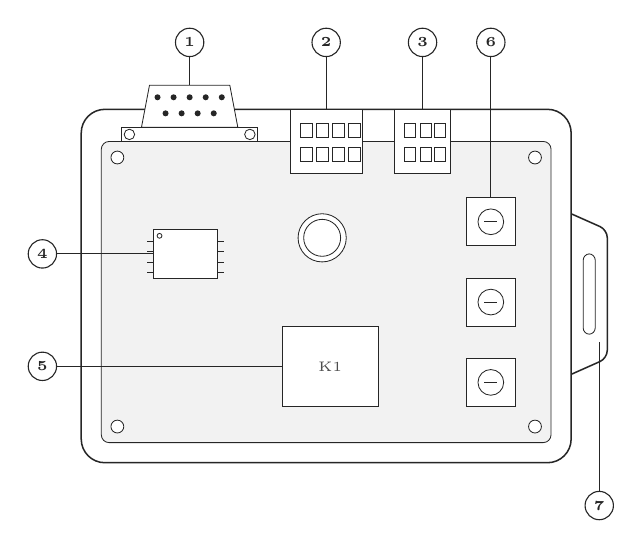
\begin{tikzpicture}[x=0.51mm,y=0.51mm]
  % caixa e orelha
  \draw[td,fill=white,rounded corners=1mm] (122,22) -- (131,26) -- (131,58) -- (122,62);
  \draw[tdfino,rounded corners=0.8mm] (125,32) rectangle (128,52);
  \draw[td,fill=white,rounded corners=3mm] (0,0) rectangle (122,88);
  % placa
  \draw[tdfino,fill=tdfill,rounded corners=1mm] (5,5) rectangle (117,80);
  \foreach \p in {(9,9),(113,9),(9,76),(113,76)} \draw[tdfino,fill=white] \p circle (1.6);
  % DB9 macho (vista superior, flange + corpo em D)
  \draw[tdfino,fill=white] (10,80) rectangle (44,83.5);
  \draw[tdfino,fill=white] (15,83.5) -- (39,83.5) -- (37,94) -- (17,94) -- cycle;
  \foreach \x in {19,23,27,31,35} \fill[tdline] (\x,91) circle (0.75);
  \foreach \x in {21,25,29,33} \fill[tdline] (\x,87) circle (0.75);
  \draw[tdfino,fill=white] (12,81.75) circle (1.3); \draw[tdfino,fill=white] (42,81.75) circle (1.3);
  % Microfit 8 e 6
  \draw[tdfino,fill=white] (52,72) rectangle (70,88);
  \foreach \x in {54.5,58.5,62.5,66.5} {\draw[tdfino] (\x,75) rectangle ({\x+3},78.5); \draw[tdfino] (\x,81) rectangle ({\x+3},84.5);}
  \draw[tdfino,fill=white] (78,72) rectangle (92,88);
  \foreach \x in {80.5,84.5,88} {\draw[tdfino] (\x,75) rectangle ({\x+2.6},78.5); \draw[tdfino] (\x,81) rectangle ({\x+2.6},84.5);}
  % CI interface RS232 (SOIC)
  \draw[tdfino,fill=white] (18,46) rectangle (34,58); \draw[tdfino] (19.5,56.5) circle (0.6);
  \foreach \y in {47.5,50,52.5,55} {\draw[tdfino] (16.5,\y) -- (18,\y); \draw[tdfino] (34,\y) -- (35.5,\y);}
  % relé
  \draw[tdfino,fill=white] (50,14) rectangle (74,34);
  \node[font=\tiny,text=tddim] at (62,24) {K1};
  % capacitor eletrolítico
  \draw[tdfino,fill=white] (60,56) circle (6); \draw[tdfino] (60,56) circle (4.6);
  % reguladores: indutor + trimpot
  \foreach \y in {14,34,54} {
    \draw[tdfino,fill=white] (96,\y) rectangle (108,{\y+12});
    \draw[tdfino] (102,{\y+6}) circle (3.2);
    \draw[tdfino] (100.4,{\y+6}) -- (103.6,{\y+6});}
  % chamadas
  \draw[lider] (27,94) -- (27,101) node[chamada,above] {1};
  \draw[lider] (61,88) -- (61,101) node[chamada,above] {2};
  \draw[lider] (85,88) -- (85,101) node[chamada,above] {3};
  \draw[lider] (18,52) -- (-6,52) node[chamada,left] {4};
  \draw[lider] (50,24) -- (-6,24) node[chamada,left] {5};
  \draw[lider] (102,66) -- (102,101) node[chamada,above] {6};
  \draw[lider] (129,30) -- (129,-7) node[chamada,below] {7};
\end{tikzpicture}}
